\section{RC Week 3}
\subsection{Building a C++ program}
\begin{frame}{The problem of \textit{building} complex programs}
\vspace{-0.10in}
\begin{block}{\textit{Building} is different from \textit{compiling}}
	\vspace{-0.07in}
	\begin{itemize}
		\item Compiling refers to the process of translating code to binaries.
		\item Building is \textbf{piecing together} from its components.
		\item A program might depend on other package.
		\item A program might use a pre-compiled library.
		\item A program might involve more than one source files.
		\item A program might need to be built for different platform
		\item Sometimes you not only needs to build just one executable, but also documentations / test suites / libraries for the sake of other programs.
	\end{itemize}
\end{block}
\vspace{-0.15in}
\begin{block}{How complicated is Linux kernel version 3.2?}
	\vspace{-0.07in}
	\begin{itemize}
		\item 37,626 – The number of files 
		\item 15,004,006 – The number of lines of code 
	\end{itemize}
\end{block}
\end{frame}

\begin{frame}{\textit{Building} a multi-file C++ program}
\begin{block}{The golden rule}
	\vspace{0.05in}
	\textrm{\textbf{\large{Each source file (\texttt{.cpp}, \texttt{.c}) compiles independently.}}}
\end{block}
\begin{block}{The \textit{building} process}
	\vspace{0.1in}
	\centering

	% Define block styles
	\tikzstyle{decision} = [diamond, draw, fill=blue!20, 
	text width=4.5em, text badly centered, node distance=3cm, inner sep=0pt]
	\tikzstyle{block} = [rectangle, draw, fill=blue!20, 
	text width=5em, text centered, rounded corners, minimum height=4em]
	\tikzstyle{line} = [draw, -latex']
	\tikzstyle{cloud} = [draw, ellipse,fill=red!20, node distance=3cm,
	minimum height=2em]
	
	\begin{tikzpicture}[node distance = 3cm, auto, scale=0.8, every node/.style={scale=0.8}]
	% Place nodes
	\node [block] (source) {Source \texttt{.cpp}};
	\node [draw,trapezium,trapezium left angle=70,trapezium right angle=-70, above of=source, node distance=2cm] (preproc) {Preprocessor};
	\node [block, above of=preproc, node distance=2cm] (prep) {Preprocessed Source \texttt{.cpp}};
	\node [draw,trapezium,trapezium left angle=70,trapezium right angle=-70, right of=prep, node distance=3cm] (compiler) {Compiler};
	\node [block, right of=compiler] (object) {Objects files \texttt{.o}};
	\node [block, below of=object] (outside) {Other Objects \texttt{.o}};
	\node [draw,trapezium,trapezium left angle=70,trapezium right angle=-70, right of=object] (linker) {Linker};
	\node [block, right of=linker] (executable) {exactuable};
	%\node [block, below of=decide, node distance=3cm] (stop) {stop};
	% Draw edges
	%\path [line] (source) -- (compiler);
	\path [line] (source) -- (preproc);
	\path [line] (preproc) -- (prep);
	\path [line] (prep) -- (compiler);
	\path [line] (compiler) -- (object);
	\path [line] (object) -- (linker);
	\path [line] (outside) -- (linker);
	\path [line] (linker) -- (executable);
	\end{tikzpicture}
\end{block}
\end{frame}

\begin{frame}{The \texttt{g++} tool chain}
\begin{block}{\texttt{g++} as a all-in-one tool}
	\vspace{-0.07in}
	\begin{itemize}
		\item Preprocessor, compiler and linker used to be separate.
		\item Now \texttt{g++} combines them into one.
		\item By default \texttt{g++} takes source files and generate executable.
		\item Using different switches you can perform individual step.
	\end{itemize}
\end{block}
\vspace{-0.15in}
\begin{block}{Options for \texttt{g++}}
	\vspace{-0.07in}
	\begin{description}[-O\{0123\}]
		\small
		\item[-o out] Name the output file as \texttt{out}. Outputs \texttt{a.out} if not present.
		\item[-std=] Specify C++ standard. Recommend \texttt{-std=c++11}.
		\item[-Wall] Report all warnings.
		\item[-O\{0123\}] Optimization level. \texttt{-O2} is the recommended for release.
		\item[-c] Only compiles the file (Can not take multiple arguments).
		\item[-E] Only pre-processes the file (Can not take multiple arguments).
	\end{description}
\end{block}
\end{frame}

\begin{frame}[fragile]{An example}
This example contains a ``main" source file accompanied with multiple other source files. All files are compiled separately into object files. We link some of them together and see what happens.

\vspace{0.04in}
\textit{Keep in mind variables/function must be first declared before used.}

\vspace{0.04in}
\texttt{$-->$ code/rc3build/main.cpp}
\inputminted{c++}{code/rc3build/main.cpp}
\end{frame}

\begin{frame}[fragile]{An example}
\label{example:dec_def}
\vspace{0.04in}
\texttt{$-->$ code/rc3build/odd.cpp}
\inputminted{c++}{code/rc3build/odd.cpp}

\vspace{0.04in}
\texttt{$-->$ code/rc3build/even.cpp}
\inputminted{c++}{code/rc3build/even.cpp}

\vspace{0.04in}
\texttt{$-->$ code/rc3build/sum.cpp}
\inputminted{c++}{code/rc3build/sum.cpp}
\end{frame}

\begin{frame}[fragile]{An example}
\texttt{$-->$ code/rc3build/prod.cpp}
\inputminted{c++}{code/rc3build/prod.cpp}

\vspace{0.04in}
\begin{small}
	The following file is a C source file. This file is given just for you to know you can do pretty weired things if you know the deal.
\end{small}

\texttt{$-->$ code/rc3build/sum\_large.c}
\inputminted{c++}{code/rc3build/sum_large.c}

\end{frame}

\begin{frame}[fragile]{An example}
We compile the source files one by one. 
\begin{minted}{text}
$ g++ -o main.o -c main.cpp
$ g++ -o odd.o -c odd.cpp
$ g++ -o even.o -c even.cpp
$ g++ -o sum.o -c sum.cpp
$ g++ -o prod.o -c prod.cpp
\end{minted}
Next one is compiled through gcc
\begin{minted}{text}
$ gcc -o sum_large.o -c sum_large.c
\end{minted}

Next step we are going to link (some of) them and execute it. Linking in \texttt{g++} is easy. If you supply \texttt{.o} files, \texttt{g++} will know that is should link them instead of compiling them.

Pay extra attention to compiler errors (actually linker errors), they are the most interesting part.

\end{frame}

\begin{frame}[fragile]{An example}
Now first standard examples
\begin{minted}{text}
$ g++ -o main main.o even.o sum.o && ./main
$ g++ -o main main.o even.o prod.o && ./main
$ g++ -o main main.o odd.o prod.o && ./main
\end{minted}

Now what if we link both \texttt{even.o} and \texttt{odd.o}
\begin{minted}{text}
$ g++ -o main main.o odd.o even.o prod.o && ./main
\end{minted}

Now what if we link both \texttt{prod.o} and \texttt{sum.o}
\begin{minted}{text}
$ g++ -o main main.o odd.o sum.o prod.o && ./main
\end{minted}

Now what if we leave out both \texttt{even.o} and \texttt{odd.o}
\begin{minted}{text}
$ g++ -o main main.o prod.o && ./main
\end{minted}

Now what if we leave out the \texttt{main.o} 
\begin{minted}{text}
$ g++ -o main even.o prod.o && ./main
\end{minted}

\end{frame}

\begin{frame}[fragile]{An example}
\framesubtitle{Surprises}

Now we introduce something crazy. The name of the function in \texttt{sum\_large.c} is really strange. But we just ignores that link its object file any way.
\begin{minted}{text}
$ g++ -o main main.o even.o sum_large.o && ./main
\end{minted}

Well it worked. The question is how on earth can this work. In fact \texttt{g++} is doing some crazy renaming when compiling your source code. The reason why they did this is understandable when you think about it in the later period of the course. 

Understanding linking actually allows you to do some crazy things. Try compiling the following file (with only one line of code) on your machine. 
\begin{minted}{text}
int main[-1u] = {1};
\end{minted}

It tooks quite long to finish. How large is the executable?

\end{frame}

\begin{frame}{Headers and inclusion}
\begin{block}{\texttt{\#include<>} : Why we need them?}
	\begin{itemize}
		\item Things must be declared before used.
		\item Each source file compiles independently. Needs a method to ``export" functions defined in one file to other files.
		\item Avoid repeating declarations. 
	\end{itemize}
\end{block}
\begin{block}{Preprocessing}
	\begin{itemize}
		\item Preprocessing is purely \textbf{textual}. 
		\item \texttt{\#include} simply copy the content.
		\item \textit{Conditional compilation directives }simply deletes unused branch. (\texttt{\#ifdef}, \texttt{\#ifndef}, \texttt{\#else}, ...)
	\end{itemize}
\end{block}

\end{frame}

\begin{frame}[fragile]{Header guards}
\framesubtitle{problem}
Whenever there is dependence of source files, there will be dependence of headers.

Consider the following \texttt{a.cpp}, \texttt{a.h}, \texttt{b.h} and \texttt{c.h}. Keep in mind that \textit{everything in C++ is allowed to have at most 1 definition during compilation.}

\begin{columns}
	\column{.5\textwidth}
	$-->$ \texttt{a.cpp}
\begin{minted}{c++}
#include "a.h"
#include "b.h"
int main() {...}
\end{minted}
	\column{.5\textwidth}
$-->$ \texttt{point.h}
\begin{minted}{c++}
struct Point{
    int x, y;
}
\end{minted}
\end{columns}
\vspace{0.2in}
\begin{columns}
	\column{.5\textwidth}
	$-->$ \texttt{a.h}
\begin{minted}{c++}
#include "point.h"
int area(Point a, Point b);
\end{minted}
\column{.5\textwidth}
$-->$ \texttt{b.h}
\begin{minted}{c++}
#include "point.h"
void circle(Point o, int r);
\end{minted}
\end{columns}
\end{frame}

\begin{frame}[fragile]{Header guards}
\framesubtitle{Solution}
The idea is to use a unique macro to guard a header.
\begin{itemize}
	\item Define that unique macro when the header is first included.
	\item Check if the macro is defined in future inclusion.
\end{itemize}

Now \texttt{point.h} becomes:

\begin{minted}{c++} 
#ifndef _POINT_H_
#define _POINT_H_
struct Point {int x, y;}
#endif
\end{minted}

The macro could be something else. Just don't use something common.

\end{frame}

\begin{frame}{Build systems}
\structure{The need for a build system}
\begin{itemize}
	\item Build process is complicated, avoid type every command.
	\item Project have dependence, need to manage dependence
	\item Compile minimum amount of code possible upon update.
	\item Many other reasons, abstract out actual compiler, compile for different platform / target.
\end{itemize}
\structure{Choices of build systems}
\begin{description}[GNU/make]
	\item[GNU/make] Our choice of make system. It has a very long history.
	\item[CMake] A modern make system used by CLion and many other projects. Very flexible and reliable. It is also a cross platform solution.
	\item[MSBuild] Build system used by Visual Studio.
\end{description}
\end{frame}

\begin{frame}{\textit{Makefile} and it's syntax}
\structure{The \textit{Makefile}}
\begin{itemize}
	\item The executable for GNU/make is simply \texttt{make}
	\item \texttt{make} requires a file that describes the building process. Such file is named \texttt{Makefile}. 
	\item \texttt{Makefile} is made up of \textit{targets}. A target can depend on other target, or some file.
\end{itemize}
\structure{Syntax}

The following syntax defines a target. Note the \texttt{tab} key.

\vspace{0.1in}

\texttt{\textit{TargetName} : Dep1 Dep2 file1.o file2.o}

\texttt{\keys{\tab} \textit{Command1-to-run}}

\texttt{\keys{\tab} \textit{Command2-to-run}}

\end{frame}

\begin{frame}{\textit{Makefile} : Example}
This is a \texttt{Makefile} for our previous example.
\texttt{$-->$ code/rc3build/Makefile}
\inputminted{c++}{code/rc3build/Makefile}
\end{frame}

\subsection{Misc of C++}
\begin{frame}{Standardized C++}
Once upon the time, programming languages are just conventions, design choices made by the language creator. 

\structure{The standardize process}
\begin{itemize}
	\item Establishes program syntax, what are acceptable and what are syntax errors?.
	\item Language semantics, what's the ``meaning" of an expression / language construct.
	\item Behavior, what are the expected behavior and what are undefined and left to the choice of compilers ...
	\item Standard library, what to include and what's the implementation constraint.
\end{itemize}
The latest standard is C++17 (3/21/2017). Major standards are C++98, C++03, C++11, C++14. C++ after C++11 is generally considered ``modern C++". 
\end{frame}

\begin{frame}{Online reference for \texttt{std::to\_string()}}
The following information comes from \texttt{http://www.cplusplus.com/reference/string/to\_string/}
\begin{figure}
	\centering
	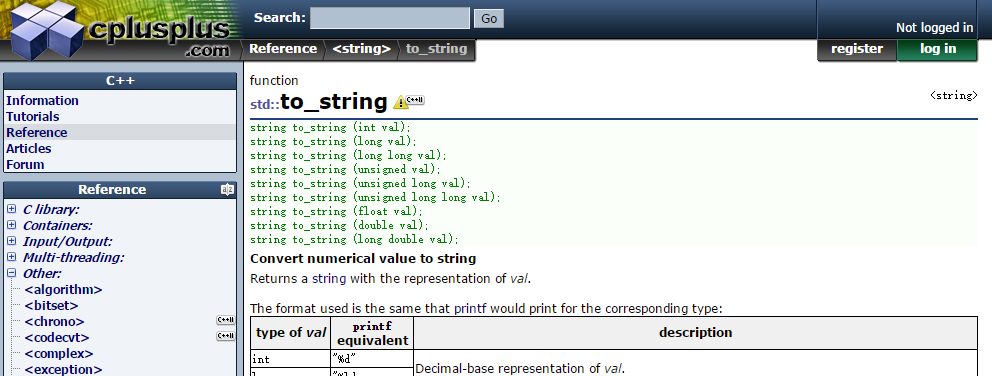
\includegraphics[scale=0.4]{fig/rc3_tostring}
	\caption{Online reference for \texttt{C++11} library function \texttt{to\_string}}
	\vspace{-0.2in}
\end{figure}

\begin{itemize}
	\item Notice the \texttt{C++11} sign.
	\item Notice the overloads supported by this function.
\end{itemize}
\end{frame}

\begin{frame}{\textit{Undefined Behaviors}}
One outcome from the standardize process is that, almost every true-or-false question about the C++ program can be answered with one of the following decisively. It is either YES, NO, or more importantly \textbf{undefined behavior} (\textit{UB} for short).

Undefined behaviors are program whose output depends on a specific platform, or a specific implementation of the compiler. You should always remember the following:
\begin{itemize}
	\item It's an absolute waste of time trying to figure out what will happen given an code that contains UB.
	\item It's dangerous and to write code that contains UB.
	\item Anyone who test you with UB, is both stupid and ignorant.
\end{itemize}

There is a reason why UB exists. It's not that the committee doesn't know how to eliminate them, but they leave room for pretty impressive \textit{compiler optimizations}.
\end{frame}

\begin{frame}{Undefined Behaviors}
Any (zero or more) of the following may happen if you trigger any of undefined behaviors:

\begin{itemize}
	\item The compiler may refuse to compile.
	\item The compiler still compiles, but throw you an warning
	\item The compiler compiles silently.
	\item Your program crashes when executed.
	\item Your program malfunctions when executed.
	\item The compiler deletes all your photos.
	\item 72 fairies come out of your screen and dance around you.
	\item \textbf{\textcolor{red}{Your program works perfectly.}}
\end{itemize} 

\textbf{It's your job to avoid UB}. We may refuse to answer the ``why my program works locally but crashes on OJ" type of question.
\end{frame}

\begin{frame}[fragile]{Undefined Behaviors}
\framesubtitle{dCommon cases}


- Integer overflow (No, it's not guaranteed to be negative!)
\begin{minted}{c++}
int x = INT_MAX; x++; 
\end{minted}

- Dereferencing \texttt{nullptr} (No, it's not guaranteed to be crash!)
\begin{minted}{c++}
int* x = nullptr; *x = 2;
\end{minted}

- Array out-of-bound (Even taking address is UB!)
\begin{minted}{c++}
int x[10] = {0};  x[10] = 1; int* x = &(x[11]);
\end{minted}



- Dangling references (You could still get correct value)
\begin{minted}{c++}
int* x = int[10]; x[3] = 5; delete[] x; cout << x[3]; 
int* f(int t) {return &t;} int* x = f(10); cout << *x;
\end{minted}

- Evaluation order and side effect :)
\begin{minted}{c++}
int i = 0; i = i++; // Yes that's UB
int j = i++ + ++i; // Yes that's UB too
f(j = i, i = j); // That's right UB again.
\end{minted}

\end{frame}

\begin{frame}{\textit{Declaration} versus \textit{Definition}}
	This whole discussion is based on one fact. 
	\begin{itemize}
		\item C++ is \textit{statically typed}
		\item Type of every identifier must be known when used.
		\item This ``identifier" includes functions, variables and arrays ...
		\item However the actual implementation can be specified later.
		\item A \textit{declaration} is a statement about what the type of an identifier (variable / function) is. 
		\item A \textit{definition} is a statements about what that object actually is. That is how much memory it consumes, what's it's data.
	\end{itemize}
	
	You have met declarations and definitions in Page.\ref{example:dec_def}.
	\texttt{extern int numbers[];} and \texttt{int reduce(int n[], int s);} are examples of declarations. The actual definition is in another file.
	
	The \texttt{extern} keyword, why is it there? 
\end{frame}

\begin{frame}[fragile]{Function \textit{signature} / \textit{prototype} and \textit{definition}}
A declaration for a function is called a function prototype. The ``type" of a function is called it's \textit{signature}. (Technically the ``signature" is not the ``type", but that's the idea.)

How much information do you need to describe the function?
\begin{itemize}
	\item The name, we need to be able to refer to that function
	\item Return type, the ``codomain" of the function.
	\item Number of inputs and their type. ``domain" of the function.
	\item Formal parameter name.
\end{itemize}

Combining them, the standard form of a function declaration will be:
\begin{minted}{c++}
ReturnType functionName(T1 arg1, T2 arg2, ...);
\end{minted}
I guess you are quite familiar with it. Note a definition of a function automatically introduce it's declaration (so the rule that everything must be declared before used is still intact).
\end{frame}

\begin{frame}[fragile]{Example}
Now a really simple example. Consider writing a declaration for the following \texttt{add} function.
\begin{minted}{c++}
int add(int x, int y) {return x + y;}
\end{minted}
No doubt above is a function definition. We first write
\begin{minted}{c++}
int add(int x, int y);
\end{minted}
Well, that's a right answer. But we could also do
\begin{minted}{c++}
int add(int elephant, int haskell);
\end{minted}
Suprised? Well it makes sense since changing formal arguments doesn't change the function at all! $f(x) = x$ and $f(z) = z$ are the same function. But we could push this even further!
\begin{minted}{c++}
int add(int, int);
\end{minted}
This will work as well, Why? This kind of declaration will be useful when you learn about function pointers.
\end{frame}

\begin{frame}[fragile]{\textit{lval} and \textit{rval}}
Compare the following 2 expression, suppose \text{arr} is an array of integers
\begin{enumerate}
	\item \mintinline{c}{arr[10]}
	\item \mintinline{c}{arr[10] + arr[1]}
\end{enumerate}
They both have the type \texttt{int} of course. 
\begin{itemize}
	\item \mintinline{c}{int *p = &(arr[10]);} makes sense.
	\item \mintinline{c}{int *p = &(arr[10] + arr[1]);} gives you compile error.
\end{itemize}  
Further more
\begin{itemize}
	\item \mintinline{c}{arr[10] = 10;} makes sense.
	\item \mintinline{c}{arr[10] + arr[1] = 20;} doesn't
\end{itemize} 
Clearly the two expression are ``different" in some sense. How? Think about memory! The first kind is called \textit{left values} and the second is called \textit{right values}. (Those are not technical definitions.)
\end{frame}

\begin{frame}[fragile]{References}

\textit{What we discuss here applies only to non-const references!}

Lvals always corresponds to a fixed memory region. This gives rises to a special construct called \textit{references}. 

\begin{minted}{c++}
int a = 1, b[10] = {2};
int& ra = a; int& rb3 = b[3];
a = 10; /* ra reads 10 */ ra = 20; // a reads 20
\end{minted}

Think about references as aliases. Essentially, you are giving the memory region associated with \texttt{a} an extra name \texttt{ra} (memory region given by \texttt{b[3]} an extra name \texttt{rb3}). 

Try resist the temptation to think reference as an \textbf{alias of variables}, but remember they are alias for the \textbf{memory region}.

References must be \textit{bind} to a memory region when created. There is no way to \textit{re-bind} of an existing reference. 
\end{frame}

\begin{frame}[fragile]{Function argument passing}
Syntacticly there exists 2 ways of argument passing:

\structure{Pass-By-Value}
\begin{minted}{c++}
int f(int x) { return (x = 2);}
\end{minted} 

\structure{Pass-By-Reference}
\begin{minted}{c++}
int g(int& x) { return (x = 2);}
\end{minted} 

We give the following code to demonstrate their difference:
\begin{minted}{c++}
int y = 10; f(y); cout << y; // returns 2, outputs 10
int z = 10; g(z); cout << z; // returns 2, outputs 2
\end{minted}
From a language point of view, reference parameter allows the function to change the input parameter. 

Some would argue there exists a third way of argument passing. 
\begin{minted}{c++}
#define SQR(x) (x * x)
\end{minted}
They have a point. We call this pass-by-name. But we choose to ignore that in this course.

\end{frame}

\begin{frame}[fragile]{Function argument passing}
Remember we are discussing how C++ manages memory. Keep in mind a memory oriented point of view is of utter importance.

We comment these two in terms of memory:
\begin{itemize}
	\item Using the pass by reference, the formal argument would be a reference to the actual argument, namely they refer to the same memory region.  
	\item Using the pass-by-value, the formal argument would be an independent \textit{copy} of actual argument. 
\end{itemize}

Pass-by-reference sounded like that it is related to pointers. This is true, in many implementations, pass-by-reference is implemented through pointers.

In pass-by-value, the word ``copy" is extremely interesting. The fact that we need to ``copy" the argument, give rise to serious problems in the later sections of this course. 
\end{frame}

\begin{frame}{Function argument passing}
This memory point of view discussion give rise to some argument:
\begin{itemize}
	\item Reference introduce an extra layer of indirect access to the original memory object, which drags down the performance.
	\item Pass-by-value needs to copy the argument, which can be slow.
\end{itemize}

In light of these observation, we suggest the following:

\begin{itemize}
	\item Small types (\texttt{int}, \texttt{float}, \texttt{char*}...) better passed by value. The cost of indirect access is much more than copying them.
	\item Complicated structure, especially large ones, or class object, better passed through reference.
\end{itemize}

On the other hand, references allows the function to change the parameter, and sometimes would like to enforce invariance of arguments. This will be solved later.
\end{frame}

\begin{frame}[fragile]{Memory layout for \textit{array} and \textit{struct}}
\begin{columns}
	\column{.5\textwidth}
	\structure{Array}
	
	Arrays are arranged in a consecutive way in memory. 
	
	Consider \texttt{int x[6];}. Each \texttt{int} costs 4 bytes. 

\vspace{.2in}
\begin{bytefield}[leftcurly=., leftcurlyspace=0pt]{16}
	\bitheader[endianness=little]{0,4,8,12}\\
	\begin{leftwordgroup}{0x90}
		\bitbox{16}{Random data...}
	\end{leftwordgroup}\\
	\begin{leftwordgroup}{0xA0}
		\bitbox{4}{\texttt{x[0]}}\bitbox{4}{\texttt{x[1]}}
		\bitbox{4}{\texttt{x[2]}}\bitbox{4}{\texttt{x[3]}}
	\end{leftwordgroup}\\
	\begin{leftwordgroup}{0xB0}
		\bitbox{4}{\texttt{x[4]}}\bitbox{4}{\texttt{x[5]}}
		\bitbox{8}{Unknown}
	\end{leftwordgroup}\\
	\begin{leftwordgroup}{0xC0}
		\bitbox{16}{Random data...}
	\end{leftwordgroup}\\
\end{bytefield}
Note \texttt{x[i]} is always \texttt{*(x + i)}. \texttt{x} essentially holds address \texttt{0xA0}.\\

	\column{.5\textwidth}
	\structure{Structures}
	
	\textit{\small{Warning: C++ standard does not fully specify memory layout.}}
	
	Consider a structure (32bit)
\begin{minted}{c++}
struct S {
    int x, y, z; long long l1;
    S* ptr; int t[2]; 
    long long l2;
};
\end{minted}

\begin{bytefield}[leftcurly=., leftcurlyspace=0pt]{16}
	\bitheader[endianness=little]{0,4,8,12}\\
	\begin{leftwordgroup}{0xA0}
		\bitbox{4}{\texttt{x}}\bitbox{4}{\texttt{y}}
		\bitbox{4}{\texttt{z}}\bitbox{4}{-}
	\end{leftwordgroup}\\
	\begin{leftwordgroup}{0xB0}
		\bitbox{8}{\texttt{l1}}\bitbox{4}{\texttt{ptr}}
		\bitbox{4}{t[0]}
	\end{leftwordgroup}\\
	\begin{leftwordgroup}{0xC0}
		\bitbox{4}{\texttt{t[1]}}\bitbox{4}{-}\bitbox{8}{\texttt{l2}}
	\end{leftwordgroup}\\
\end{bytefield}
\end{columns}
\end{frame}

\begin{frame}[fragile]{Remarks on arrays}
Arrays are passed by passing the address of its first element. That \textbf{address is copied}, in this sense the actual content of the array is passed as references. 



You might wonder the difference of the following 2: 

\begin{minted}{c++}
int foo(int x[], int size);
int foo(int *x, int size);
\end{minted}

In practice there aren't any (if not templates).

Remember the following expression does \textbf{NOT} make sense:
\begin{minted}{c++}
int foo(int x[size]);
\end{minted}

Whenever you need to pass an array as an argument, remember to \textbf{pass it's size along with it}! 

\small{Footnote: In fact C++ considers the size of the array part of its type, meaning C++ believes for \texttt{int x[3];} and \texttt{int y[4];}, \texttt{x} and \texttt{y} has different type. It's just happens that both types can be converted into \texttt{int*} when passed as argument. See \texttt{code/rc3arr/run.sh}}
\end{frame}

\begin{frame}{Remarks on structures}
\begin{itemize}
	\item \texttt{sizeof} a struct is NOT the sum of \texttt{sizeof} its members.
	\item Structures arrange its members in the order of declaration.
	\item Members of a structure are put in the continuous region.
\end{itemize}

You need to think structures as a new type: structures a models a new type of data, a new concept. It is a \textbf{compound type}.

If you pass an structure by value, and if there is an array embedded in the structure, the array will be copied. This makes sense since the array is considered part of the value of the new datatype.

In C++, structures are simply ``\texttt{class}"es with one change : members of a structure are by default \texttt{public}. This implies classes follows the same set of rules in terms of memory layouts.

We omit the discussion on pointers of structure.
\end{frame}

\begin{frame}[fragile]{Initialization of Arrays}
The rules of initialization is extremely complicated in C++, this is due to two (competing) reasons:
\begin{itemize}
	\item C++ tries to keep backward compatibility with C. 
	\item C++ needs a unified modern syntax to initialize things.
\end{itemize}
This gets even more complicated if you take into account the fact that \texttt{struct}s are essentially same as \texttt{class}es. 

\textbf{These rules applies also to \texttt{new}/\texttt{new[]} operator}.

We first consider initializing an array:
\begin{minted}{c++}
int arr0[5] = {1, 2, 3, 4, 5}; 
int arr1[5] = {1, 2}; // {1, 2, 0, 0, 0};
int arr2[5] = {1}; // {1, 0, 0, 0, 0};
int arr3[5] = {0}; // {0, 0, 0, 0, 0};
int arr4[] = {1, 2, 3} // arr4[3] = {1, 2, 3}; useful!
int arr5[3]{1, 2}; // {1, 2, 0}; c++11 style;
int arr6[3]{}; // {0, 0, 0}; c++11 style;
\end{minted}
\end{frame}

\begin{frame}[fragile]{Initialization of structures}

\begin{columns}
	\column{.5\textwidth}
	Consider \texttt{struct S}:
\begin{minted}{c++}
struct S {
    int x, y;
    int arr[2];
    double d;
};
\end{minted}
You might need to specify \texttt{-std=c++11} when using these initializations.

Now think about it, how to initialize \texttt{S sarr[2];}?

	\column{.5\textwidth}
	\structure{Curly-brace enclosed initializer}
\begin{minted}{c++}
S s1 = {1, 2, 3, 4, 1.0};
S s2 = {1, 2, {3, 4}, 1.0};
\end{minted}
We recommend the second one.
	
\structure{Default constructor}
\begin{minted}{c++}
S s1{};
\end{minted}
This initializes all fields to zero.

\structure{In-place}
\begin{minted}{c++}
struct P {
    int x = 1, y = 2;  
    int arr[2] = {3 , 4}; 
    double d = 1.0;
};
\end{minted}
\end{columns}
\end{frame}

\begin{frame}[fragile]{Function arguments: pointers or references?}
We have one last question. Consider the following code:
\begin{minted}{c++}
struct S {int arr[100];};
void foo(S* s); void bar(S& s):
\end{minted}
Now two functions are functionally same, which should I perfer?

\begin{itemize}
	\item Pro-ref: References guarantees non-\texttt{null}, which is safer.
	\item Pro-ptr: Pointers allow \texttt{nullptr}, allows for the idea like "not-applicable" or "default value".
	\item Pro-ref: References good for \textit{ownership}, semantically clear.
	\item Pro-ref: Syntactically cleaner. No need to modify call sites.
	\item Pro-ptr: References are used like values, not intuitive. Readers of the code has to jump to decl. Example \texttt{std::getline}.
	\item Pro-ref: Pointers are easily confused with array.
	\item Pro-ptr: Pointers are the only way to work with array. (If you ignore \texttt{std::vector}).
\end{itemize}
\end{frame}

\begin{frame}{References as an abstraction}
We would like to quote the following words from the standard:
\begin{quotation}
	References are not objects; they do not necessarily occupy storage, although the compiler may allocate storage if it is necessary to implement the desired semantics.
\end{quotation}
In this way references are kind of special, since all usual types are connected to some memory: an \texttt{int} is 4 bytes and there is a 32-bit binary value in those 4 bytes. Pointer are addresses, they occupies 4 bytes in the memory and there is a 32-bit address in those 4 bytes. 

Reference is defined through \textit{abstraction}: We have a contract with the language on how this thing should behave, but we make no assumption on how the compiler achieve such effect. Compiler could choose to use pointers to achieve references, but on the other hand it doesn't have to. 
\end{frame}

\begin{frame}[fragile]{Size of a reference type}
\begin{itemize}
	\item References are often implemented by pointers.
	\item Now what is the size of the reference type.
\end{itemize}
Now \texttt{sizeof(int\&)} will not work. Std. requires \texttt{sizeof} the reference type returns \texttt{sizeof} the referenced type, \texttt{sizeof(int)}.

But we could try
\begin{minted}{c++}
struct S {int x; int& y;} cout << sizeof(S);
\end{minted}
Will this work? Consider the code on the left side. Output?
\vspace{-0.15in}
\begin{columns}
	\column{.5\textwidth}
\begin{minted}{c++}
struct S {int x; int& y};
int main() {
    int a = 3;
    S s = {a, a};
    cout << sizeof(s);
} 
\end{minted}
	\column{.5\textwidth}
	
	\structure{It could be 8}
	
	Implemented by pointers, 4 bytes.
	
	\structure{It could be 4}
	
	Compiler discovered it is not used. This also obeys the std.
	
	\structure{It could be 5, 6, 7, 9, 120. Why?}
\end{columns}
\end{frame}


